\documentclass[12pt, letterpaper]{article}
\usepackage[titletoc,title]{appendix}
\usepackage{booktabs}
\usepackage{caption}
\newcommand\fnote[1]{\captionsetup{font=small}\caption*{#1}}

\usepackage[dvipsnames,svgnames,table]{xcolor}
\definecolor{dark-red}{rgb}{0.75,0.10,0.10}
\usepackage[margin=1in]{geometry}
\usepackage{graphicx}                % Handles inclusion of major graphics formats and allows use of
\usepackage{amsfonts,amssymb,amsbsy}
\usepackage{amsxtra}
\usepackage{natbib}
\usepackage{verbatim}
\setcitestyle{round,semicolon,aysep={},yysep={;}}
\usepackage{setspace}		     % Permits line spacing control. Options are \doublespacing, \onehalfspace
\usepackage{sectsty}		     % Permits control of section header styles
\usepackage{lscape}
\usepackage{fancyhdr}		     % Permits header customization. See header section below.
\usepackage{url}                 % Correctly formats URLs with the \url{} tag
\usepackage{fullpage}		     %1-inch margins
\usepackage{multirow}
\usepackage{rotating}
\setlength{\parindent}{3em}
\usepackage{subcaption}
\usepackage[T1]{fontenc}
\usepackage{bm}
\usepackage{lmodern}

\usepackage{chngcntr}
\usepackage[linkcolor=dark-red,
			colorlinks=true,
			urlcolor=blue,
			pdfstartview={XYZ null null 1.00},
			pdfpagemode=UseNone,
			citecolor={dark-red},
			pdftitle={Face of Crime in Prime Time}]{hyperref}
\newcommand{\EpisodeCount}{731}
\newcommand{\VictimCount}{1,578}
\newcommand{\CriminalCount}{1,117}
\newcommand{\MajorCrimeEpisodeCount}{659}
\newcommand{\OriginalEpisodeCount}{151}
\newcommand{\OriginalVictimWhitePct}{73.4}
\newcommand{\OriginalVictimBlackPct}{10.4}
\newcommand{\OriginalVictimHispanicPct}{14.6}
\newcommand{\OriginalVictimFemalePct}{40.3}
\newcommand{\OriginalCriminalWhitePct}{84.0}
\newcommand{\OriginalCriminalBlackPct}{11.2}
\newcommand{\OriginalCriminalHispanicPct}{4.3}
\newcommand{\OriginalCriminalFemalePct}{26.8}
\newcommand{\SvuEpisodeCount}{386}
\newcommand{\SvuVictimWhitePct}{78.1}
\newcommand{\SvuVictimBlackPct}{10.8}
\newcommand{\SvuVictimHispanicPct}{8.3}
\newcommand{\SvuVictimFemalePct}{60.9}
\newcommand{\SvuCriminalWhitePct}{81.7}
\newcommand{\SvuCriminalBlackPct}{9.9}
\newcommand{\SvuCriminalHispanicPct}{7.6}
\newcommand{\SvuCriminalFemalePct}{27.4}
\newcommand{\CriminalIntentEpisodeCount}{194}
\newcommand{\CriminalIntentVictimWhitePct}{82.1}
\newcommand{\CriminalIntentVictimBlackPct}{9.3}
\newcommand{\CriminalIntentVictimHispanicPct}{3.7}
\newcommand{\CriminalIntentVictimFemalePct}{42.7}
\newcommand{\CriminalIntentCriminalWhitePct}{86.4}
\newcommand{\CriminalIntentCriminalBlackPct}{7.7}
\newcommand{\CriminalIntentCriminalHispanicPct}{3.6}
\newcommand{\CriminalIntentCriminalFemalePct}{31.9}
\newcommand{\NcvsSeriousBlackLowPct}{19.1}
\newcommand{\NcvsSeriousBlackHighPct}{21.1}
\newcommand{\NcvsRapeBlackLowPct}{15.0}
\newcommand{\NcvsRapeBlackHighPct}{17.0}
\newcommand{\NcvsAssaultBlackLowPct}{19.0}
\newcommand{\NcvsAssaultBlackHighPct}{22.4}
\newcommand{\UcrMurderVictimBlackLowPct}{48.3}
\newcommand{\UcrMurderVictimBlackHighPct}{48.8}
\newcommand{\NcvsSeriousFemaleLowPct}{47.1}
\newcommand{\NcvsSeriousFemaleHighPct}{48.3}
\newcommand{\NcvsRapeFemaleLowPct}{88.7}
\newcommand{\NcvsRapeFemaleHighPct}{89.7}
\newcommand{\UcrMurderVictimFemaleLowPct}{21.8}
\newcommand{\UcrMurderVictimFemaleHighPct}{22.3}


\title{\Large{The Face of Crime in Prime Time:\\ Evidence from Law and Order}\footnote{Data and scripts behind the analysis presented here can be downloaded at: \url{https://github.com/notnews/face_of_crime}.}}

\author{Gaurav Sood\thanks{Gaurav can be reached at \href{mailto:gsood07@gmail.com}{\footnotesize{\texttt{gsood07@gmail.com}}}} \and Daniel Trielli\thanks{Daniel is a professional journalist. He can be reached at: \href{mailto:dtrielli@gmail.com}{\footnotesize{\texttt{dtrielli@gmail.com}}}}\vspace{.5cm}}

\date{}

\begin{document}
\maketitle

\begin{comment}

setwd(paste0(basedir, "face_of_crime/ms"))
tools::texi2dvi("face_of_crime.tex", pdf=TRUE, clean=TRUE)
setwd(basedir)

\end{comment}


\begin{abstract}
\noindent We tally the coded race and gender of victims and criminals in \EpisodeCount{} episodes of three Law \& Order series. The share of classified criminal characters coded Black is \CriminalIntentCriminalBlackPct\% in \textit{Criminal Intent}, \SvuCriminalBlackPct\% in \textit{Special Victims Unit}, and \OriginalCriminalBlackPct\% in the sampled seasons of the original series. These shares are below the historical arrest benchmarks. The corresponding Black victim shares are \CriminalIntentVictimBlackPct\%, \SvuVictimBlackPct\%, and \OriginalVictimBlackPct\%, below the share in the historical serious-violent-victimization benchmark. Women are more common among coded criminal characters than among people arrested for the compared offenses. The comparisons describe these episodes and the available historical reference series; they do not measure what viewers learned from watching them.
\end{abstract}
\clearpage
\setstretch{2}

Offensive portrayals of African Americans on entertainment shows have long been the norm in the US. For instance, minstrel shows, popular in the 19th century and the first half of the 20th century, regularly portrayed African Americans as lazy and dim-witted \citep{dates1993split, toll1974blacking}. More recently, \citet{entman2001black} found that 56\% of blacks in the media were portrayed as violent compared to 11\% of the whites.

There is good reason to think that these offensive portrayals reinforce negative stereotypes of African Americans. For at least some people likely take these portrayals as representative of African Americans \citep[see][]{punyanunt2008perceived}. Correspondingly, research suggests that belief in aversive racial stereotypes is associated with exposure to television programming \citep{busselle2002television, entman2001black, armstrong1992tv}. For instance, exposure to television news is correlated with the extent to which college students endorse that blacks are lazy \citep{busselle2002television}. Similarly, \citet{armstrong1992tv} find that more television news the college students consumed, more likely they were to believe that blacks have lower socio-economic outcomes. (Albeit, ``TV drama exposure was associated with beliefs that Black Americans had a relatively higher socio-economic standing.'') A more comprehensive study of how blacks are portrayed in the media by \citet{entman2001black} reached similar conclusions---exposure to nonfictional portrayals of African Americans is associated with negative stereotypes of blacks.

Television's role in perpetuating negative stereotypes is worrisome because of how consequential stereotypes are in shaping attitudes, preferences, and behavior. Much research shows that racial stereotypes shape political attitudes \citep[see, for e.g.,][]{sniderman1995scar, hurwitz1997public, peffley1997racial, dixon2006psychological} and affect economic behavior \citep[see, for e.g.,][]{bertrand2004emily}.

Given the concern, numerous researchers study how blacks are covered on various television programs \citep[for e.g.,][]{entman2001black, eschholz2004images}. One particular focus of the effort---given blacks are stereotyped as violent and criminal, and given the impact such stereotypes may have on policy consequential attitudes related to punitiveness---has been on describing the extent to which blacks are overrepresented as criminals, especially as violent criminals.

Studies on the extent to which blacks are overrepresented in crime news or other programming about crime suggest that the bias is generally small but very variable---some studies document a modest anti-black bias in some news programs in some areas of the country \citep{gilliam1996crime}, while others document a large anti-white bias (when compared to criminal arrest data, which are likely biased in favor of whites) \citep{chiricos2002racial, dixon2000overrepresentation, eschholz2004images} (see Table \ref{tab:lit}).

\begin{table}[p]
\centering
\scriptsize
\caption{Racial distribution of perpetrators and victims in earlier television studies}
\label{tab:lit}
\begin{tabular}{p{.12\linewidth}p{.09\linewidth}p{.12\linewidth}p{.40\linewidth}p{.12\linewidth}}
\toprule
Region & Period & Media & Finding & Citation \\
\midrule
Hampton Roads, Virginia & Jan. 3-31, 2011 & Local TV News & Perpetrators: 50.7\% Blacks (Violent Crime), 75\% Whites (White Collar Crime),  75.9\% Blacks (General Crime) (Graph 4)

Victims: 78.3\% White (Violent Crime), 82.1\% Whites (General Crime) (Graph 5) & \citet{leadbleed2011} \\
National & 1994--1997, 2000 & Network News & Perpetrators:

All Crime: 71\% White (vs. 68\% in Uniform Crime Reports),  27\% Blacks (vs. 30\% in Uniform Crime Reports) (Table 4)

Violent Crime: 48\% White (vs. 56\% in Uniform Crime Reports), 38\% Blacks (vs. 42\% in Uniform Crime Reports) (Table 5)

Victims:
All Crime: 51\% White (vs. 28\% in Uniform Crime Reports),  30\% Blacks (vs. 48\% in Uniform Crime Reports) (Table 6) & \citet{dixon2003portrayal}  \\
National & 2002--2003 & Local TV News & Perpetrator (All Crime): 26.82\% White, 21.06\% Black, 42.27\% Not Indicated

Victim (All Crime): 27.88\% White,  9.24\% Black, 56.97\% Not Indicated (Table 1) & \citet{bjornstrom2010race} \\
National & 2000--2001 & NYPD Blue and Law and Order & NYPD Blue:

Offender:  50\% Whites (vs. 68\% in Uniform Crime Reports),  38\% Blacks, 11\%

Violent Off./Sus. 43\% (black) 46\% (white) 10\%

Law and Order Figures don't add up to 100. (Table 1) & \citet{eschholz2004images} \\
Washington, D.C. & May and June 2005 & Local TV News & Perpetrators:
Violent Crime: 9\% Whites, 32\% Blacks, 51\% Unrevealed

Non-violent Crime: 14\% Whites, 29\% Blacks, 50\% Unrevealed

Victims:

Violent Crime: 15\% White,  10\% Blacks, 72\% Unrevealed

Non-violent Crime: 3\% White,  7\% Blacks, 83\% Unrevealed & \citet{gross2006covering} \\
Los Angeles & 1995--1996 & Local TV News & All Perpetrators: 37\% Black (versus 21\% in California Department of Justice Criminal Profile or CDJCP), 21\% (versus 28\% in CDJCP) (Table 4)

Felons: 44\% Black (versus 25\% in CDJCP), 18\% (versus 23\% in CDJCP) (Table 5) & \citet{dixon2000overrepresentation} \\
Los Angeles & 1993--1994 & Local TV News (KABC) & No commensurate numbers, except: 40\% where race identified (purportedly across all crime stories). Where race identified in violent crime stories: 45\% White and in non-violent crime: 75\% white.

Blacks actual crime rate: 2.8 * share of population. Coverage: 3.2 * share of population. (Assuming the coverage is estimated as percentage where race identified and not as percentage of total mentions) (Figure 2)

Non-violent crime: Whites overrepresented by nearly 400\% (see Figure 3) & \citet{gilliam1996crime} \\
Orlando & 1998 & Local TV News & All Crime: 18\% Black (Versus 42\% Arrest Rate),  65\% White (Versus 58\% Arrest Rate) (Table  3)

Violent Crime: 20\% Black (Versus 49\% Arrest Rate), 61\% White (Versus 51\% Arrest Rate)(Table  3) & \citet{chiricos2002racial} \\
\bottomrule
\end{tabular}
\end{table}


In this paper, we add to this body of work. We tally the gender and race of criminals and victims depicted in three Law \& Order series and compare their composition with historical arrest records, victim surveys, and population data. The series, offense categories, places, and years differ across those sources, so the comparisons describe the coded portrayals in context.

\section*{Learning from Television}
Mass media is an important part of the information environment for many people. Thus, what is covered in the media tends to affect what people believe \citep{gerbner1986living, shanahan1999television}. For instance, exposure to more vivid violent media causes people to think that crime and police immorality are more common in the real world \citep{riddle2010always}. Similarly, the extent to which a topic is covered on television news affects how important people think it is \citep{mccombs1972agenda, iyengar2010news, iyengar1990accessibility}.

Similar mechanism likely holds when someone watches one of the tens of hundreds of crime dramas on television. A person watching a crime drama, aware of its fictional nature, may still inadvertently think that the drama accurately `mirrors' society. For instance, people perceive negative personality traits of African Americans portrayed on television as true to life \citep{punyanunt2008perceived}. These inference are liable to be encouraged by prior interpretation and acceptance of flawed---because they are imprecise---statements such as `art reflects life' as true.

Increasingly common mass-media tropes such as realism in depiction and explicit statements designed to cue realism may also increase the chances that people take fictional portrayals as reasonably accurate depictions of reality. As a case in point, all Law \& Order \textit{Special Victims Unit} series episodes start with the statement: ``\ldots In New York City, the dedicated detectives who investigate these vicious felonies are members of an elite squad known as the Special Victims Unit. These are their stories.'' It is not unreasonable to think that some people listening to the statement may come to think that the crimes covered in the drama represent a broad, perhaps representative, set of all ``sexually based crimes.''

Besides learning about the extent of crime and what kind of crime is prevalent from television, people may also learn associations between kinds of people and criminal activity, especially when people involved are (superficially) distinctive---say, in the color of their skin. The logic goes that if certain kinds of people are frequently shown as perpetrators of crime, people may come to believe that as large a share of perpetrators belongs to that group. By the same token, over-representation of certain groups as victims may promote misleading views of what populations are the most vulnerable to crime.

\section*{Data and Measurement}
The data are from three Law \& Order series: Original Law \& Order series (Original), Law \& Order: Special Victims Unit (SVU), and Law \& Order: Criminal Intent (Criminal Intent). All the three shows are police procedurals set in New York City. Criminal Intent, which ran between 2001--2011, purportedly follows detectives of the `Major Case Squad,' a division of the New York Police Department (NYPD) focused on solving major crimes against rich, famous, or important people. Meanwhile SVU, which has been on television since 1999, purportedly follows detectives of the NYPD division devoted to handling ``sexually based offenses,'' the `Special Victims Unit.'

The three series were long-running television programs. The episode coding in this study covers the original series in 1990--1991 and 2005--2010, Criminal Intent in 2001--2011, and SVU in 1999--2016. The original audience-data script depends on files absent from this repository, so we do not report audience averages here.

For the Original series, we only have data from Seasons 1 and 2 (1990--1991) and Seasons 16--20 (2005--2010).\footnote{The choice of the seasons is a reflection of what was available on streaming on Amazon Instant as of July, 2016.} In all, we have data from \OriginalEpisodeCount{} shows. For CI, we have \CriminalIntentEpisodeCount{} coded rows across its 10 seasons, spanning 2001--2011. And for SVU, we have \SvuEpisodeCount{} coded rows spanning seasons 1--17 and broadcast years 1999--2016. In all, across the three series, we have data from \EpisodeCount{} shows, with \VictimCount{} recorded victims and \CriminalCount{} recorded criminals; the race or gender of some characters was not classified.  We coded the race and gender of all criminals and victims whose race and gender was identified.

We define criminals as characters whose guilt is very clearly indicated; our definition includes characters not convicted or even indicted for a crime. In line with the law, active instigators and financiers of crime were coded as criminals. We marked attempted crimes as such. Lastly, we focus on `major' crimes, excluding infractions such as failing to comply with court orders.

We coded victims' and criminals' race as white, black, Asian, or Hispanic, following the general census guidelines.\footnote{\url{http://www.census.gov/topics/population/race/about.html}} Characters of Middle-Eastern descent were coded as white, but a note marking their specific background was included in the data. And under `Hispanics,' we included non-Hispanic Latinos such as Brazilians.

In addition to the data on the race and gender of the victims and the criminals from the shows, we collected data on a few baselines. From the 1990, 2000, and 2010 census, we collected data on the percentage of whites, blacks, and men in the US and in New York City. Like \citet{dixon2000overrepresentation}, from the Federal Bureau of Investigation's Uniform Crime Report (UCR), we gathered data on the percentage of blacks, whites and men arrested for \textit{All Crimes}, \textit{Violent Crimes}, and \textit{Sexually Based Crimes}. From New York Police Department's Crime and Enforcement Activity in New York City Report (NYPD),\footnote{\url{http://www.nyc.gov/html/nypd/html/analysis_and_planning/crime_and_enforcement_activity.shtml}} we gathered data on the percentage of blacks, whites and Hispanics who were suspected of (and were victims of) murder, rape, assault and robbery each year between 2008 and 2015. Lastly, from the Bureau of Justice Statistics' National Crime Victimization Survey (NCVS) \citep{powers2016national, victimization1998national}, we gathered data on the race and gender of victims of crime.

The UCR data on race of alleged criminals is available for 1995--2015. In UCR, race is split into white, black, American Indian or Alaskan Native, Asian, and Native Hawaiian or Other Pacific Islander. The totals in these categories include Hispanics. Data on Hispanic background only began to be collected in 2013, and even then the race totals are not split by Hispanic ethnicity. Not separating out Hispanics naturally inflates the numbers for whites and blacks. But the inflation for blacks is quite modest. Nearly 93\% of Hispanics self-identify as whites \citep{steffensmeier2011reassessing}. And accounting for Hispanics changes the percentage of blacks rape and assault by generally no more than a couple of percentage points \citep[see figure 4,][]{steffensmeier2011reassessing}.\footnote{\citet{steffensmeier2011reassessing} adjust UCR data by leveraging arrest data from California and New York, where arrest data includes Hispanics.} Thus, for the main analyses, which focus on representation of blacks and Hispanics, we utilize unadjusted numbers for blacks from UCR.

In UCR, 28 types of crimes are split into two categories: \textit{Violent Crime} and \textit{Property Crime}. \textit{Violent Crime} includes murder and non-negligent manslaughter, rape, robbery, and aggravated assault. And \textit{Property Crime} includes burglary, larceny-theft, motor vehicle theft, and arson. We collected data on the percentage of people arrested by race (white and black) and gender (male) for all crimes, violent crimes, as well as arrested for three of the most common offenses shown in the Law \& Order shows: homicides, rapes, and assaults. (\MajorCrimeEpisodeCount{} of \EpisodeCount{} shows or just over 90\% of the shows included in our data featured a rape, murder, or assault.)

Victim data from the NCVS covers the period between 1993--2014. Racial data in the NCVS can be gathered with Hispanics included in the category totals, and without. We collected both kinds of data, but focus on data that more closely matches our data for Law \& Order, and separates out Hispanics.

Like the UCR, the NCVS aggregates various crimes into categories. In NCVS, however, the categories are \textit{Violent Victimization} and \textit{Serious Violent Victimization}. Both account for victims of rape, sexual assault, and robbery. \textit{Violent Victimization}, however, tallies all types of assault, while \textit{Serious Violent Victimization} only tallies aggravated assaults. Therefore, \textit{Serious Violent Victimization} is the closest to the \textit{Violent Crime} category in the UCR. Hence, we use data from that category. In addition, we also collect data for two specific offenses: rape/sexual assault and aggravated assault. Given that the NCVS data comes from interviews with victims, there is naturally no data on murders. Data on the race and gender of murder victims comes from UCR.\footnote{Since homicides almost always lead to the discovery of the bodies of victims, data on their gender and race are usually present. In 2015, for instance, there were 13,455 homicide victims. Of those, 29 (0.2 percent) were of an unknown gender. Thus, for data about gender of homicide victims, the percentages we use are the same offered by the UCR, which are calculated on the total of homicide victims, even the ones whose gender is unknown as that has a negligible impact on the final numbers. For instance, if we include victims with unknown gender---which is done by UCR---78.8 percent of all victims were male. Excluding those, the percentage changes to 79.0 percent. For perpetrators, we also use percentages offered by the UCR, but there is a high number of perpetrators unknown gender. Therefore, the percentages are based on the total of perpetrators whose gender is known.}

\section*{Results}
To put the racial and gender breakdown of coded Law \& Order characters in context, we compare the percentage of black and female criminals and victims on the three Law \& Order shows to a variety of baselines. In the main text, we describe the percentage of black and female criminals and victims by show, same percentages for episodes featuring murder, and SVU episodes featuring rape. (Criminal Intent and Original had fewer than 10 episodes each where rape was one of the crimes.) We compare these to average percentage of black, Hispanic, and female criminals for all crimes, rape, and murder from the UCR, and percentage of black and female victims for murder, rape, and serious violent crimes over the available historical years. A series of graphs and tables in ~\ref{si_figs} and ~\ref{si_tabs} break data down by year, and provide other baselines like data from the census that we don't include in the main text.

As Figures~\ref{fig:perp_race} and \ref{fig:perp_race_hispanic} show, the classified criminal characters are predominantly white: \CriminalIntentCriminalWhitePct\% in Criminal Intent, \SvuCriminalWhitePct\% in SVU, and \OriginalCriminalWhitePct\% in Original. The Black shares are \CriminalIntentCriminalBlackPct\%, \SvuCriminalBlackPct\%, and \OriginalCriminalBlackPct\%, respectively. These descriptive shares are lower than the corresponding historical arrest shares in the reference series. Arrests measure enforcement, not all crimes committed, and the crime mix differs between shows and benchmarks.

The annual Black criminal shares fluctuate across broadcast years (Figure~\ref{fig:perp_race_ts} and Table~\ref{tab:c_race}). The table also shows changes in the historical rape-arrest series around the FBI's 2012 definition change. Those values cannot by themselves isolate the effect of the definition change or provide a matched comparison with the shows.

\begin{figure}[!htbp]
\centering
\caption{Share of Black Criminals in Law \& Order and Historical Reference Series}
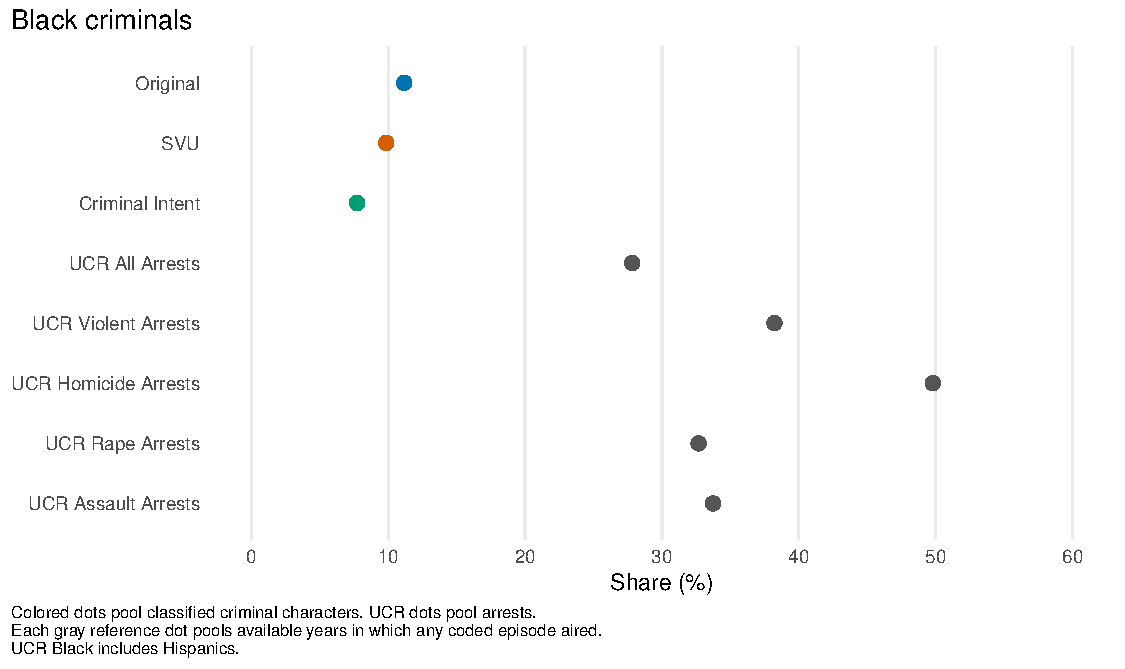
\includegraphics[width=\linewidth]{../figs/all_criminals_by_race.pdf}
\label{fig:perp_race}
\end{figure}

\begin{figure}[htbp]
\centering
\caption{Share of Hispanic Criminals in Law \& Order and Historical Reference Series}
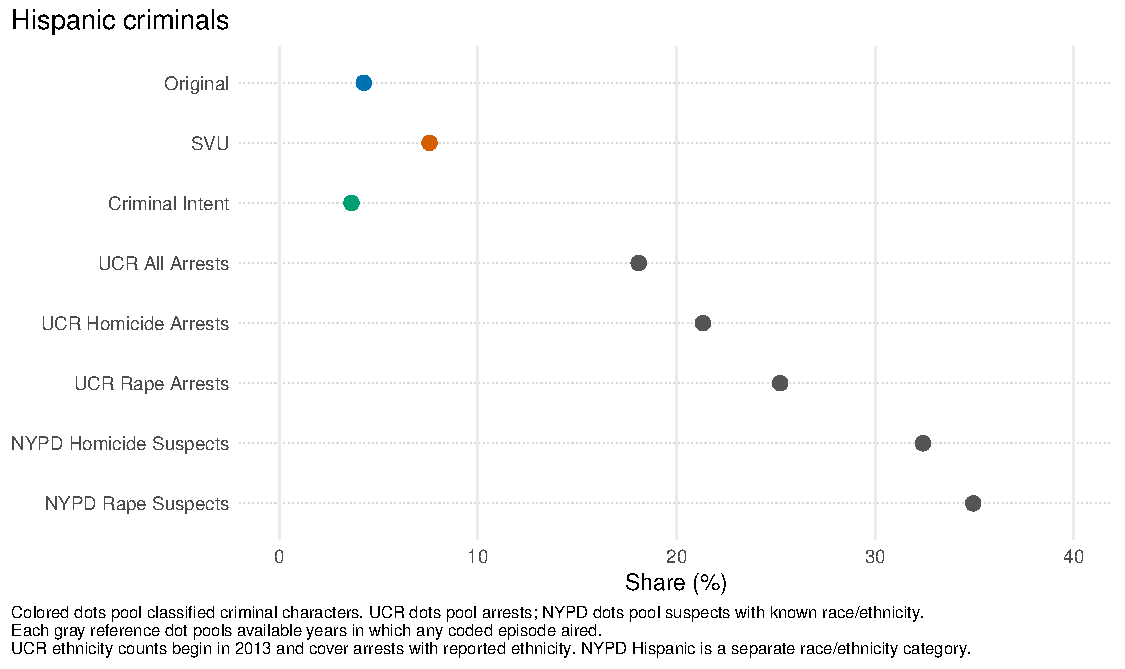
\includegraphics[width=\linewidth]{../figs/all_criminals_by_race_hispanic.pdf}
\label{fig:perp_race_hispanic}
\end{figure}

White characters also account for most classified victims (Figure~\ref{fig:victim_race}). The Black victim shares are \CriminalIntentVictimBlackPct\% in Criminal Intent, \SvuVictimBlackPct\% in SVU, and \OriginalVictimBlackPct\% in Original. For comparison, the historical NCVS Black share averaged \NcvsSeriousBlackPct\% for serious violent victimization, \NcvsRapeBlackPct\% for rape or sexual assault, and \NcvsAssaultBlackPct\% for aggravated assault during 1999--2014. The UCR Black share of murder victims averaged \UcrMurderVictimBlackPct\% over the available years. These categories differ in offense mix, geography, years, and reporting process; the comparisons are descriptive rather than like-for-like estimates. Annual show values appear in Figure~\ref{fig:victim_race_ts} and Table~\ref{tab:v_race}.

\begin{figure}[htbp]
\centering
\caption{Share of Black Victims in Law \& Order and Historical Reference Series}
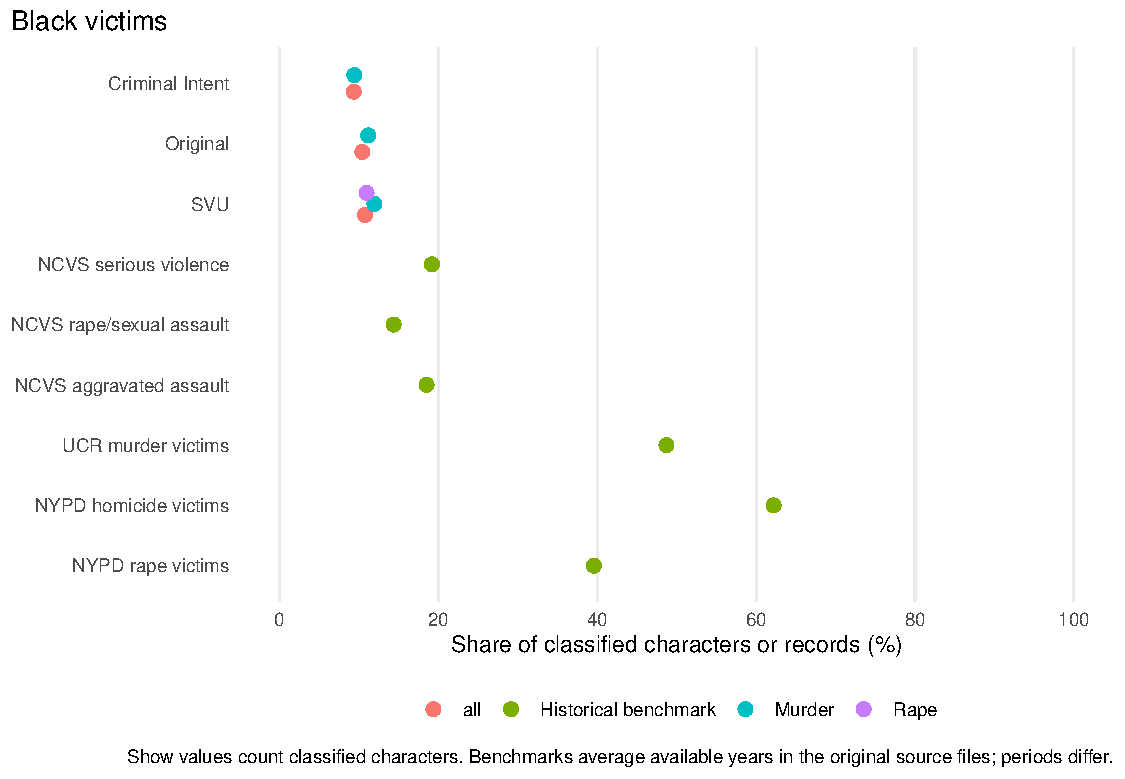
\includegraphics[width=\linewidth]{../figs/all_victims_by_race.pdf}
\label{fig:victim_race}
\end{figure}

\begin{figure}[htbp]
\centering
\caption{Share of Hispanic Victims in Law \& Order and Historical Reference Series}
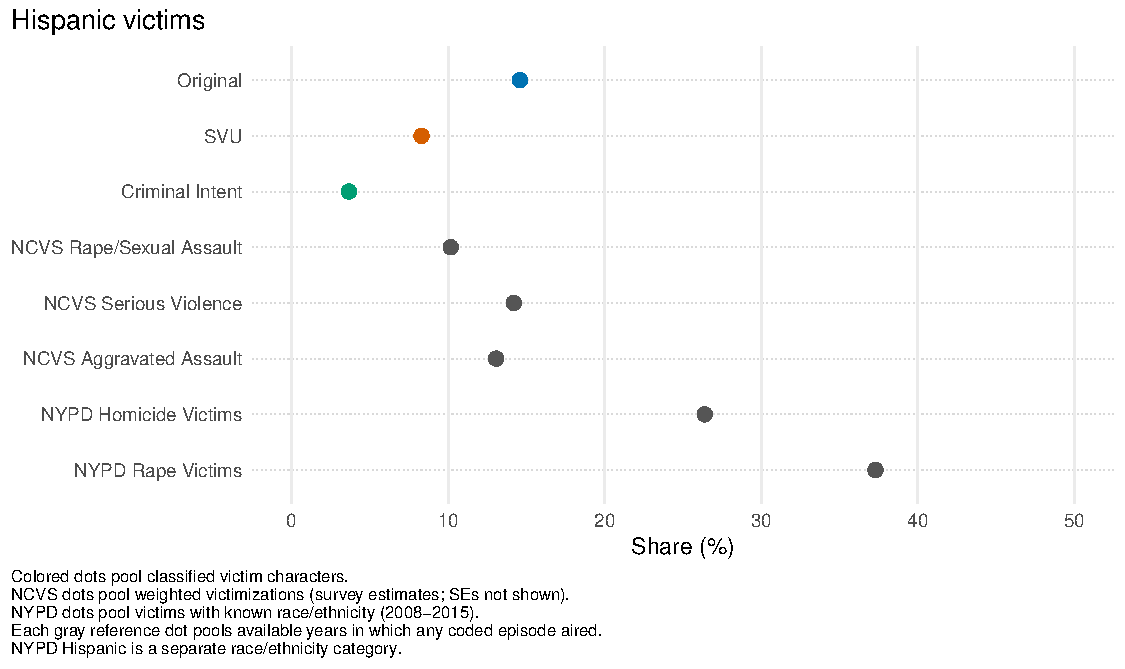
\includegraphics[width=\linewidth]{../figs/all_victims_by_race_hispanic.pdf}
\label{fig:victim_race_hispanic}
\end{figure}

Women account for \CriminalIntentCriminalFemalePct\% of classified criminals in Criminal Intent, \SvuCriminalFemalePct\% in SVU, and \OriginalCriminalFemalePct\% in Original (Figure~\ref{fig:perp_sex}). These proportions exceed the female shares in the historical UCR arrest categories shown in the figure. Annual show shares and year-specific UCR comparisons appear in Figure~\ref{fig:perp_sex_ts} and Table~\ref{tab:c_sex}.

\begin{figure}[htbp]
\centering
\caption{Share of Female Criminals in Law \& Order and Historical Reference Series}
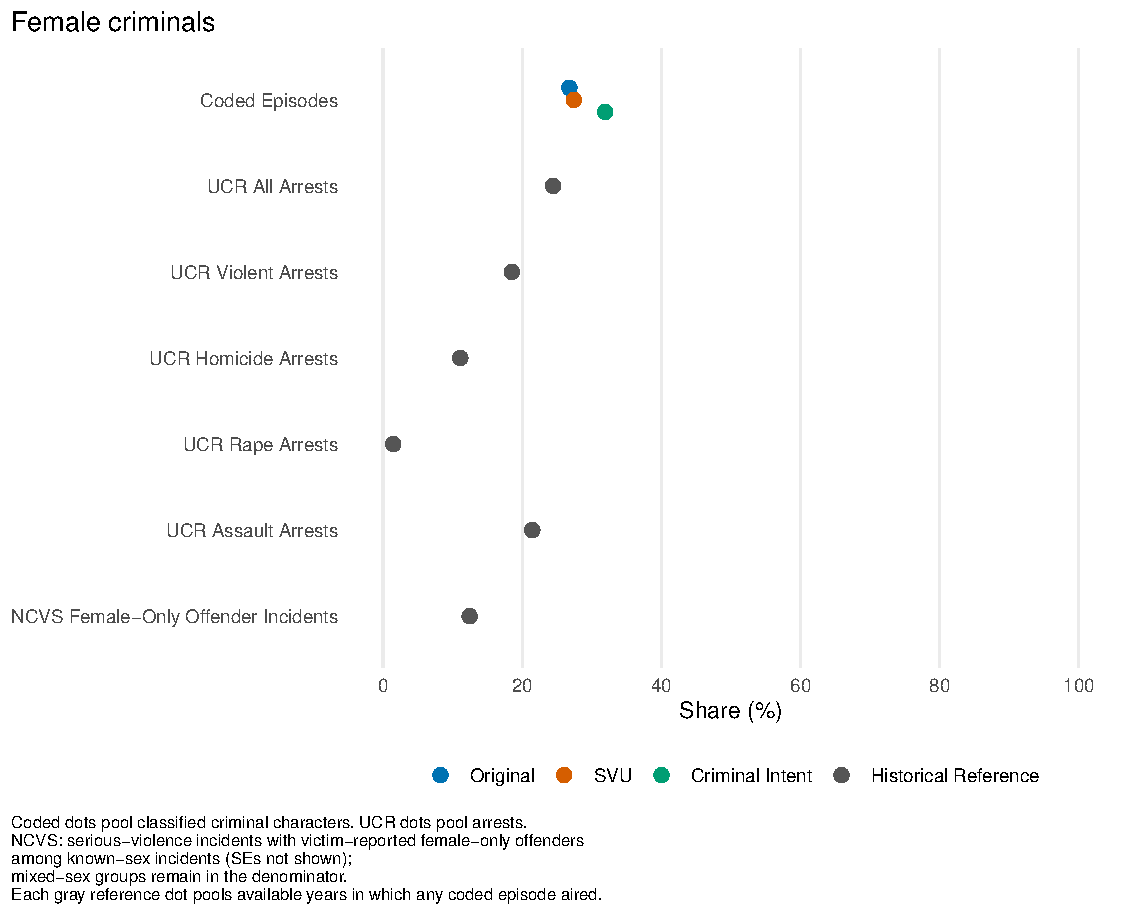
\includegraphics[width=\linewidth]{../figs/all_criminals_by_gender.pdf}
\label{fig:perp_sex}
\end{figure}

Women account for \CriminalIntentVictimFemalePct\% of classified victims in Criminal Intent, \SvuVictimFemalePct\% in SVU, and \OriginalVictimFemalePct\% in Original (Figure~\ref{fig:victim_sex}). In the historical NCVS files, women account for \NcvsSeriousFemalePct\% of serious violent victimizations and \NcvsRapeFemalePct\% of rape or sexual-assault victimizations. Their share of UCR murder victims averages \UcrMurderVictimFemalePct\%. The show and reference categories do not have the same offense mix. Annual values are shown in Figure~\ref{fig:victim_sex_ts} and Table~\ref{tab:v_sex}.

\begin{figure}[htbp]
\centering
\caption{Share of Female Victims in Law \& Order and Historical Reference Series}
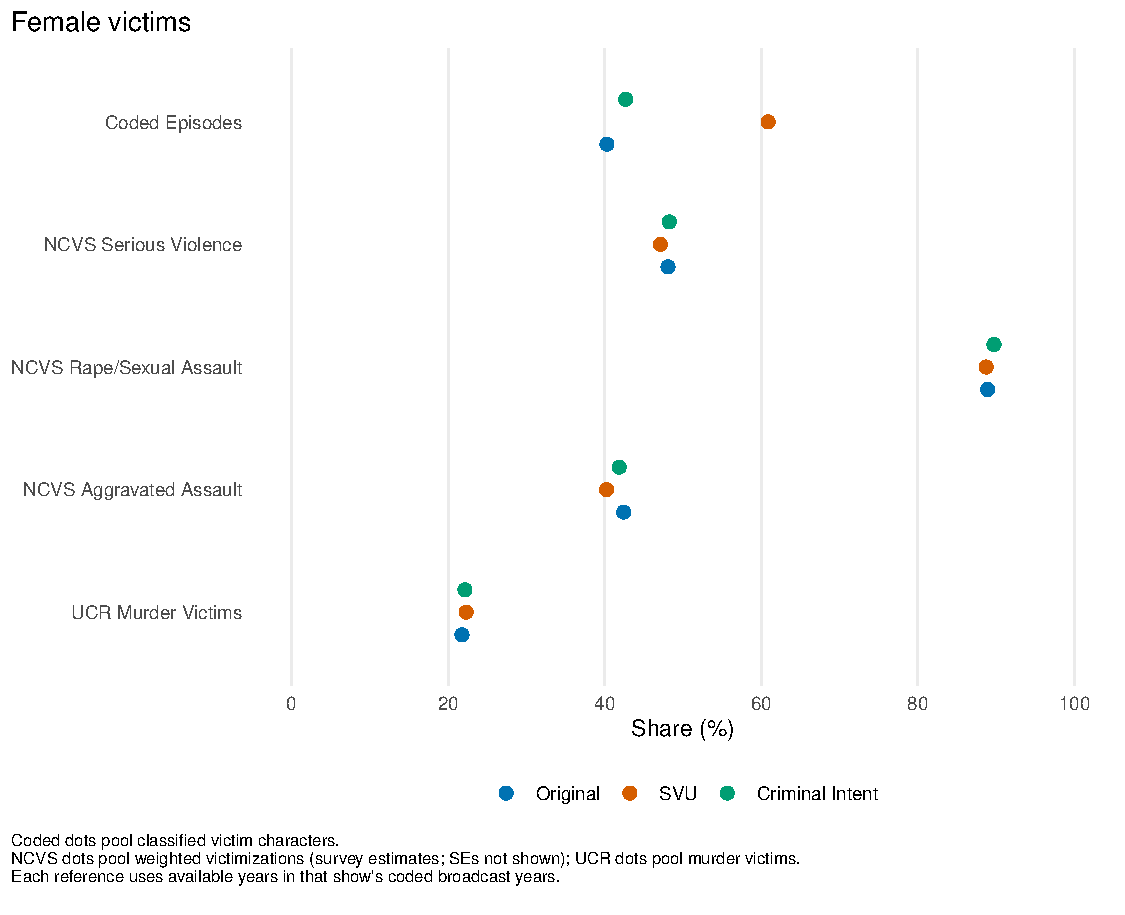
\includegraphics[width=\linewidth]{../figs/all_victims_by_gender.pdf}
\label{fig:victim_sex}
\end{figure}

\section*{Discussion}
Popular television is our bay window to the world. What we see on television likely has a sizable influence on how we think about the world. In particular, television programming likely influences how we think about crime, how common we think it is, especially in our communities, who we think perpetrates it, the reasons why criminals do what they do, who the victims are, the efficacy of the police and judicial systems, among other things.

Across these coded episodes, Black characters account for smaller shares of classified criminals and victims than the Black shares in several historical arrest and victimization series. Female criminal characters account for larger shares than women in several arrest categories. The size of each difference depends on the crime category, years, geography, and the exclusion of unclassified characters. The episode census supports claims about portrayal in these three series and sampled seasons. Whether these portrayals change viewers\textquotesingle{} beliefs remains a separate question.

Several mechanisms might produce these patterns. The series select different offenses and stories, and the characters visible in each story reflect casting and narrative choices. Writers might also have wanted to counter a viewer's confusion between $p(\text{black}|\text{criminal})$ and $p(\text{criminal}|\text{black})$ \citep[see][]{bordalo2016stereotypes, ahler2016parties}; political commitments could motivate such a choice. A commercial motive could also favor stories centered on white victims or criminals if producers expected those stories to attract viewers. We have no evidence about these production decisions or their effects on viewers, so these possibilities remain untested. The estimates here describe the coded characters in the sampled episodes.

\clearpage
\bibliographystyle{plainnat}
\bibliography{crime}


\clearpage
\appendix
\renewcommand{\thesection}{SI \arabic{section}}
\renewcommand\thetable{\thesection.\arabic{table}}
\renewcommand\thefigure{\thesection.\arabic{figure}}
\counterwithin{figure}{section}
\counterwithin{table}{section}

\begin{center}
\Large{Supporting Information}
\end{center}

\section{Percentage of Black and Female Criminals and Victims in Law \& Order By Year}
\label{si_figs}

\begin{figure}[htbp]
\centering
\caption{Race of Criminals in Law \& Order Original, SVU, and Criminal Intent by Year}
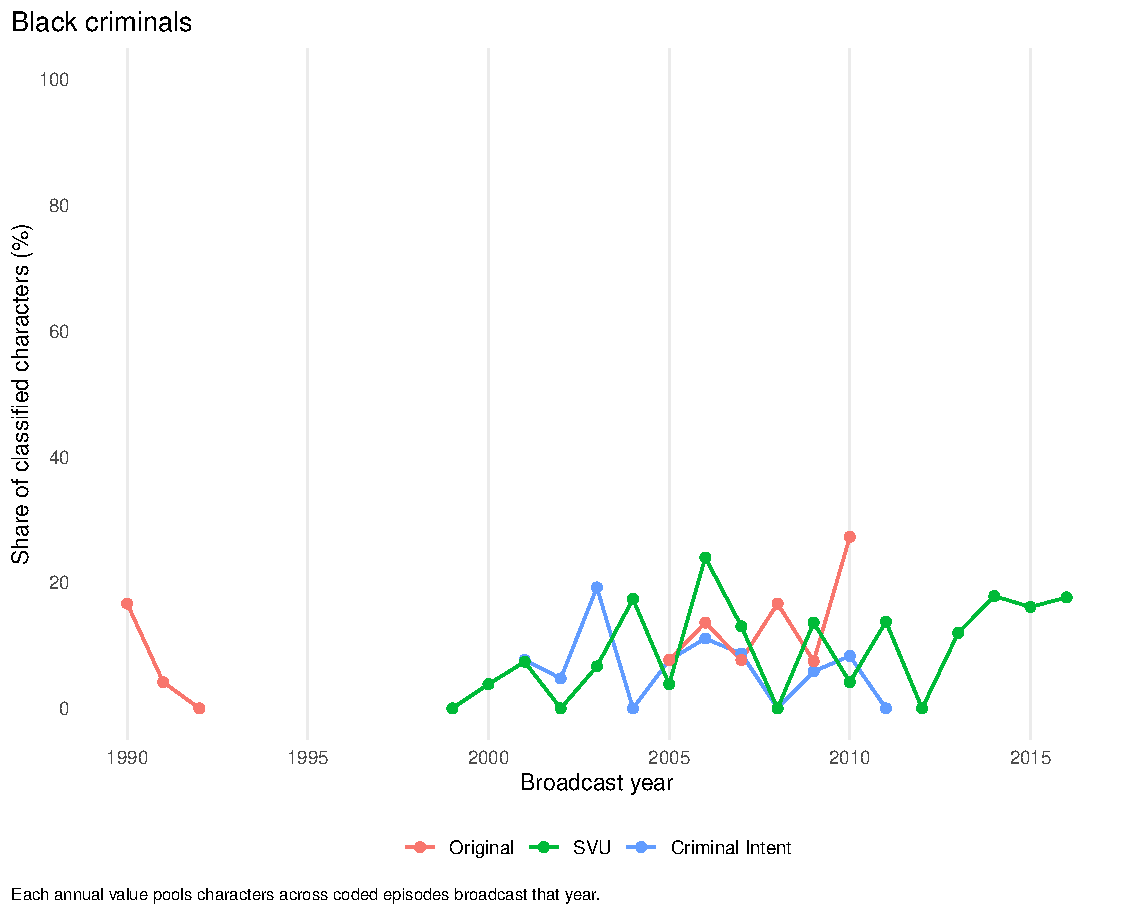
\includegraphics[width=\linewidth]{../figs/all_criminals_by_race_ts.pdf}
\label{fig:perp_race_ts}
\end{figure}

\begin{figure}[htbp]
\centering
\caption{Race of Victims in Law \& Order Original, SVU, and Criminal Intent by Year}
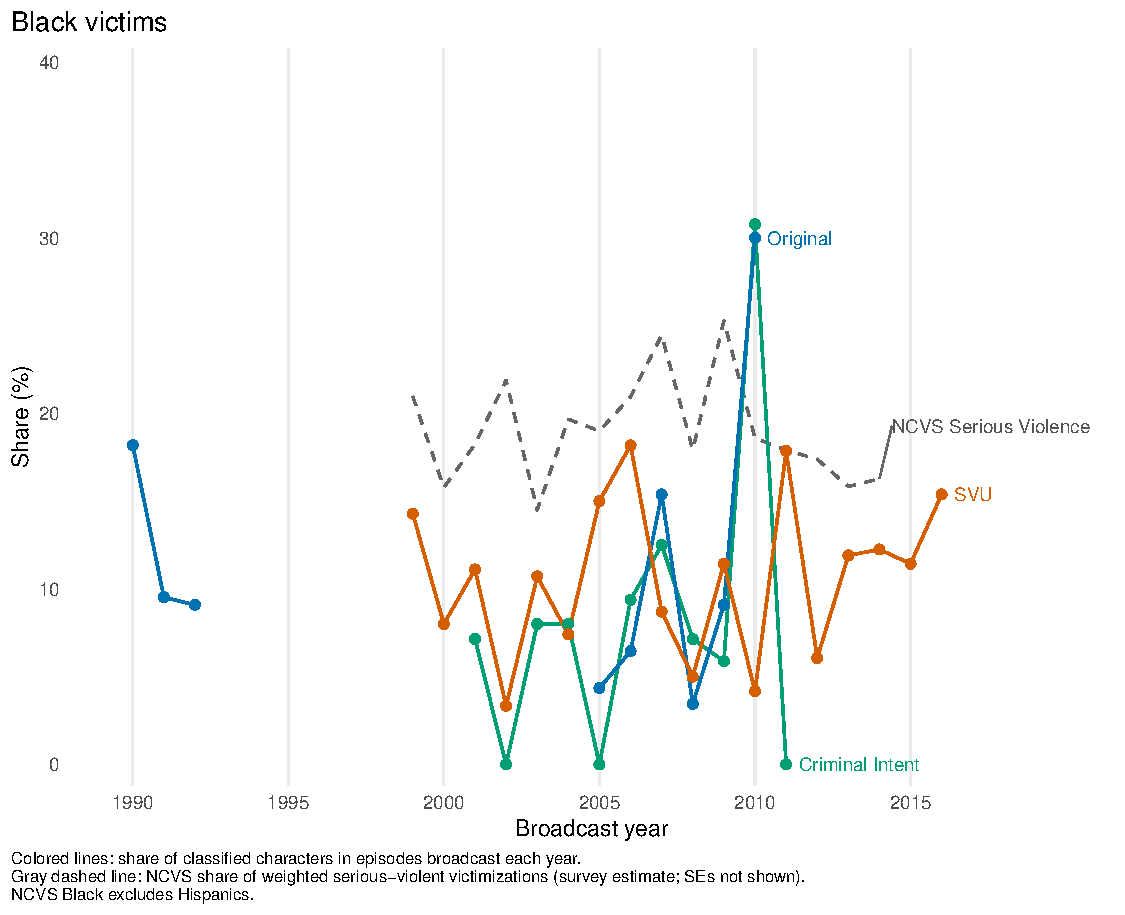
\includegraphics[width=\linewidth]{../figs/all_victims_by_race_ts.pdf}
\label{fig:victim_race_ts}
\end{figure}

\begin{figure}[htbp]
\centering
\caption{Gender of Criminals in Law \& Order Original, SVU, and Criminal Intent by Year}
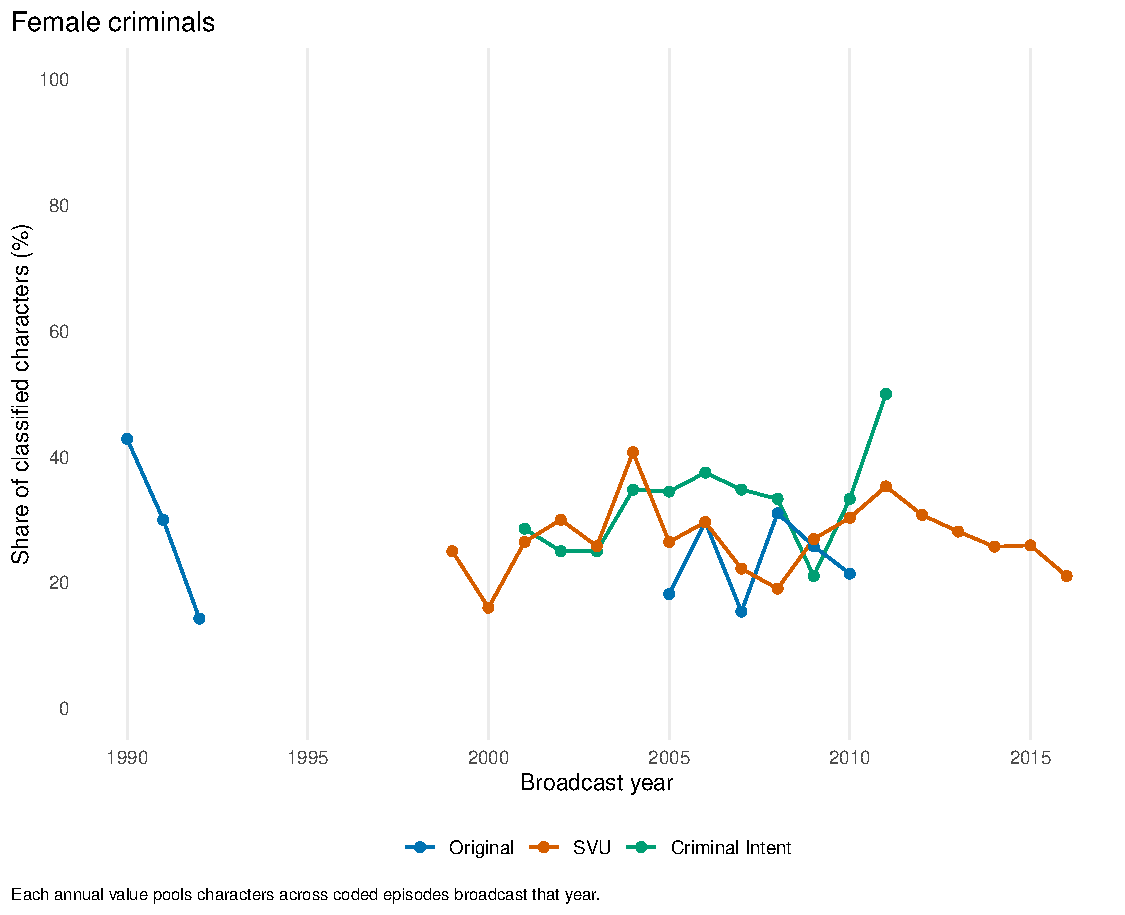
\includegraphics[width=\linewidth]{../figs/all_criminals_by_gender_ts.pdf}
\label{fig:perp_sex_ts}
\end{figure}

\begin{figure}[htbp]
\centering
\caption{Gender of Victims in Law \& Order Original, SVU, and Criminal Intent by Year}
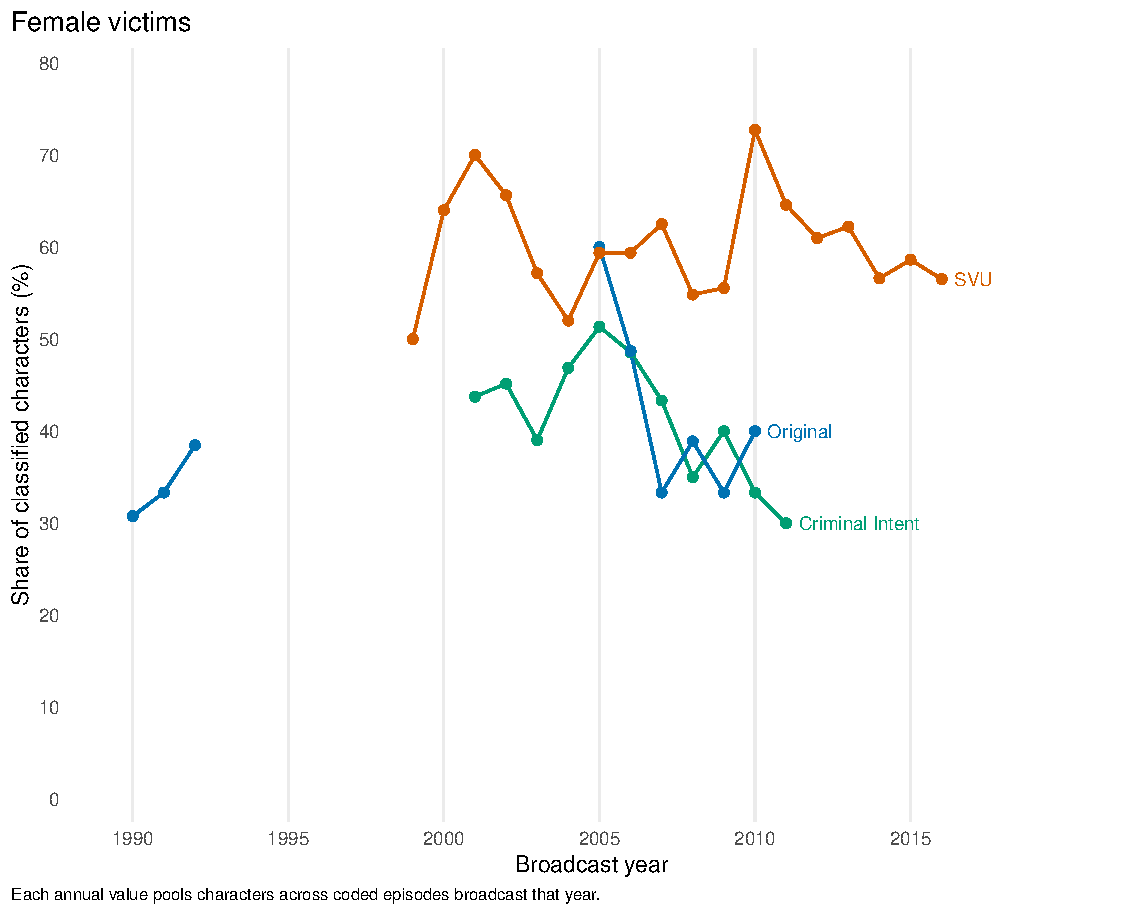
\includegraphics[width=\linewidth]{../figs/all_victims_by_gender_ts.pdf}
\label{fig:victim_sex_ts}
\end{figure}

\clearpage
\section{Sex and Race of Criminals and Victims in Law \& Order and Historical Reference Series}
\label{si_tabs}

\begin{sidewaystable}[p]
\centering
\caption{Annual share of black victim characters and historical comparisons}
\label{tab:v_race}
\scriptsize
\resizebox{\linewidth}{!}{%
\begin{tabular}{lrrrrrrrrrrr}
\toprule
Year & Criminal Intent & Original & SVU & NCVS serious violence & NCVS rape/sexual assault & NCVS aggravated assault & UCR murder victims & NYPD homicide victims & NYPD rape victims & US Census & NY Census \\
\midrule
1990 & -- & 18.2 & -- & -- & -- & -- & -- & -- & -- & 12.0 & 28.8 \\
1991 & -- & 9.5 & -- & -- & -- & -- & -- & -- & -- & -- & -- \\
1992 & -- & 9.1 & -- & -- & -- & -- & -- & -- & -- & -- & -- \\
1999 & -- & -- & 14.3 & 21.4 & 16.4 & 19.0 & 46.0 & -- & -- & -- & -- \\
2000 & -- & -- & 8.0 & 16.0 & 9.2 & 13.8 & 48.0 & -- & -- & 12.3 & 26.6 \\
2001 & 7.1 & -- & 11.1 & 19.5 & 22.1 & 18.9 & 47.0 & -- & -- & -- & -- \\
2002 & 0.0 & -- & 3.3 & 22.1 & 27.3 & 22.2 & 48.0 & -- & -- & -- & -- \\
2003 & 8.0 & -- & 10.7 & 15.2 & 7.4 & 12.6 & 48.0 & -- & -- & -- & -- \\
2004 & 8.0 & -- & 7.4 & 20.0 & 19.1 & 16.7 & 47.0 & -- & -- & -- & -- \\
2005 & 0.0 & 4.3 & 15.0 & 20.7 & 24.9 & 21.8 & 48.0 & -- & -- & -- & -- \\
2006 & 9.4 & 6.5 & 18.2 & 21.8 & 18.9 & 27.8 & 50.0 & -- & -- & -- & -- \\
2007 & 12.5 & 15.4 & 8.7 & 24.9 & 6.3 & 24.2 & 49.0 & -- & -- & -- & -- \\
2008 & 7.1 & 3.4 & 5.0 & 19.2 & 16.3 & 16.4 & 48.0 & 62.1 & 40.6 & -- & -- \\
2009 & 5.9 & 9.1 & 11.4 & 26.3 & 12.7 & 24.2 & 48.0 & 57.6 & 40.5 & -- & -- \\
2010 & 30.8 & 30.0 & 4.2 & 19.1 & 12.2 & 21.1 & 50.0 & 67.0 & 40.9 & 12.6 & 25.5 \\
2011 & 0.0 & -- & 17.9 & 18.2 & 14.7 & 18.0 & 50.0 & 61.8 & 36.8 & -- & -- \\
2012 & -- & -- & 6.1 & 17.9 & 5.6 & 18.6 & 51.0 & 60.1 & 37.9 & -- & -- \\
2013 & -- & -- & 11.9 & 16.5 & 7.7 & 20.6 & 51.0 & 62.9 & 40.8 & -- & -- \\
2014 & -- & -- & 12.2 & 17.3 & 22.6 & 15.1 & 51.0 & 62.4 & 39.7 & -- & -- \\
2015 & -- & -- & 11.4 & -- & -- & -- & 52.0 & 63.7 & 39.4 & -- & -- \\
2016 & -- & -- & 15.4 & -- & -- & -- & -- & -- & -- & -- & -- \\
\bottomrule
\end{tabular}%
}
\par\smallskip
\parbox{\linewidth}{\footnotesize Values are percentages of classified characters in the shows or percentages reported by the historical comparison files. Missing years are shown as --.}
\end{sidewaystable}


\clearpage
\begin{sidewaystable}[p]
\centering
\caption{Annual share of black criminal characters and historical comparisons}
\label{tab:c_race}
\scriptsize
\resizebox{\linewidth}{!}{%
\begin{tabular}{lrrrrrrrrrrrr}
\toprule
Year & Criminal Intent & Original & SVU & UCR all arrests & UCR violent arrests & UCR homicide arrests & UCR rape arrests & UCR assault arrests & NYPD homicide suspects & NYPD rape suspects & US Census & NY Census \\
\midrule
1990 & -- & 16.7 & -- & -- & -- & -- & -- & -- & -- & -- & 12.0 & 28.8 \\
1991 & -- & 4.2 & -- & -- & -- & -- & -- & -- & -- & -- & -- & -- \\
1992 & -- & 0.0 & -- & -- & -- & -- & -- & -- & -- & -- & -- & -- \\
1999 & -- & -- & 0.0 & 28.6 & 38.7 & 51.8 & 36.2 & 34.8 & -- & -- & -- & -- \\
2000 & -- & -- & 3.8 & 27.9 & 37.8 & 48.8 & 34.1 & 34.0 & -- & -- & 12.3 & 26.6 \\
2001 & 7.7 & -- & 7.4 & 28.1 & 37.6 & 48.7 & 34.8 & 33.7 & -- & -- & -- & -- \\
2002 & 4.8 & -- & 0.0 & 26.9 & 38.0 & 50.0 & 34.0 & 34.2 & -- & -- & -- & -- \\
2003 & 19.2 & -- & 6.7 & 27.0 & 37.2 & 48.5 & 33.3 & 33.0 & -- & -- & -- & -- \\
2004 & 0.0 & -- & 17.4 & 26.8 & 36.9 & 47.2 & 31.9 & 32.7 & -- & -- & -- & -- \\
2005 & 7.7 & 7.7 & 3.8 & 27.8 & 38.8 & 48.6 & 32.7 & 34.3 & -- & -- & -- & -- \\
2006 & 11.1 & 13.6 & 24.0 & 28.0 & 39.3 & 50.9 & 32.5 & 34.5 & -- & -- & -- & -- \\
2007 & 8.7 & 7.7 & 13.0 & 28.2 & 39.0 & 50.4 & 33.5 & 33.7 & -- & -- & -- & -- \\
2008 & 0.0 & 16.7 & 0.0 & 28.3 & 39.4 & 50.1 & 32.2 & 34.2 & 60.8 & 52.8 & -- & -- \\
2009 & 5.9 & 7.5 & 13.6 & 28.3 & 38.9 & 49.3 & 32.5 & 33.9 & 59.8 & 52.4 & -- & -- \\
2010 & 8.3 & 27.3 & 4.2 & 28.0 & 38.1 & 48.7 & 31.8 & 33.5 & 60.9 & 52.6 & 12.6 & 25.5 \\
2011 & 0.0 & -- & 13.8 & 28.4 & 38.3 & 49.7 & 32.9 & 33.6 & 56.3 & 48.8 & -- & -- \\
2012 & -- & -- & 0.0 & 28.1 & 38.5 & 49.4 & 32.5 & 34.1 & 53.7 & 50.5 & -- & -- \\
2013 & -- & -- & 12.0 & 28.3 & 38.7 & 52.2 & 31.3 & 33.9 & 55.0 & 53.0 & -- & -- \\
2014 & -- & -- & 17.9 & 27.8 & 37.7 & 51.3 & 29.9 & 33.1 & 59.8 & 49.3 & -- & -- \\
2015 & -- & -- & 16.1 & 26.6 & 36.4 & 51.1 & 28.2 & 32.1 & 62.1 & 51.2 & -- & -- \\
2016 & -- & -- & 17.6 & -- & -- & -- & -- & -- & -- & -- & -- & -- \\
\bottomrule
\end{tabular}%
}
\par\smallskip
\parbox{\linewidth}{\footnotesize Values are percentages of classified characters in the shows or percentages reported by the historical comparison files. Missing years are shown as --.}
\end{sidewaystable}


\clearpage
\begin{sidewaystable}[p]
\centering
\caption{Annual share of female victim characters and historical comparisons}
\label{tab:v_sex}
\scriptsize
\resizebox{\linewidth}{!}{%
\begin{tabular}{lrrrrrrrrr}
\toprule
Year & Criminal Intent & Original & SVU & NCVS serious violence & NCVS rape/sexual assault & NCVS aggravated assault & UCR murder victims & US Census & NY Census \\
\midrule
1990 & -- & 30.8 & -- & -- & -- & -- & -- & 51.3 & 53.2 \\
1991 & -- & 33.3 & -- & -- & -- & -- & -- & -- & -- \\
1992 & -- & 38.5 & -- & -- & -- & -- & -- & -- & -- \\
1999 & -- & -- & 50.0 & 48.2 & 93.3 & 39.2 & 24.0 & -- & -- \\
2000 & -- & -- & 64.0 & 38.1 & 96.0 & 27.1 & 24.0 & 50.9 & 52.6 \\
2001 & 43.8 & -- & 70.0 & 49.0 & 90.1 & 41.1 & 24.0 & -- & -- \\
2002 & 45.2 & -- & 65.6 & 49.3 & 86.6 & 44.0 & 23.0 & -- & -- \\
2003 & 39.0 & -- & 57.1 & 50.7 & 94.0 & 41.6 & 22.0 & -- & -- \\
2004 & 46.9 & -- & 52.0 & 45.4 & 97.6 & 37.1 & 22.0 & -- & -- \\
2005 & 51.4 & 60.0 & 59.4 & 40.1 & 92.7 & 39.3 & 21.0 & -- & -- \\
2006 & 48.6 & 48.7 & 59.4 & 47.4 & 77.6 & 42.5 & 21.0 & -- & -- \\
2007 & 43.3 & 33.3 & 62.5 & 46.5 & 95.5 & 39.0 & 22.0 & -- & -- \\
2008 & 35.0 & 38.9 & 54.8 & 54.9 & 88.7 & 47.2 & 22.0 & -- & -- \\
2009 & 40.0 & 33.3 & 55.6 & 49.4 & 93.5 & 45.0 & 23.0 & -- & -- \\
2010 & 33.3 & 40.0 & 72.7 & 52.5 & 94.4 & 43.2 & 23.0 & 50.8 & 52.5 \\
2011 & 30.0 & -- & 64.6 & 47.5 & 85.7 & 43.0 & 22.0 & -- & -- \\
2012 & -- & -- & 61.0 & 42.3 & 62.2 & 42.5 & 22.0 & -- & -- \\
2013 & -- & -- & 62.2 & 49.0 & 88.7 & 39.1 & 22.0 & -- & -- \\
2014 & -- & -- & 56.6 & 46.9 & 90.1 & 39.6 & 23.0 & -- & -- \\
2015 & -- & -- & 58.6 & -- & -- & -- & 21.0 & -- & -- \\
2016 & -- & -- & 56.5 & -- & -- & -- & -- & -- & -- \\
\bottomrule
\end{tabular}%
}
\par\smallskip
\parbox{\linewidth}{\footnotesize Values are percentages of classified characters in the shows or percentages reported by the historical comparison files. Missing years are shown as --.}
\end{sidewaystable}


\clearpage
\begin{sidewaystable}[p]
\centering
\caption{Annual share of female criminal characters and historical comparisons}
\label{tab:c_sex}
\scriptsize
\resizebox{\linewidth}{!}{%
\begin{tabular}{lrrrrrrrrrr}
\toprule
Year & Criminal Intent & Original & SVU & UCR all arrests & UCR violent arrests & UCR homicide arrests & UCR rape arrests & UCR assault arrests & US Census & NY Census \\
\midrule
1990 & -- & 42.9 & -- & -- & -- & -- & -- & -- & 51.3 & 53.2 \\
1991 & -- & 30.0 & -- & -- & -- & -- & -- & -- & -- & -- \\
1992 & -- & 14.3 & -- & -- & -- & -- & -- & -- & -- & -- \\
1999 & -- & -- & 25.0 & 21.8 & 17.0 & 11.4 & 1.3 & 19.7 & -- & -- \\
2000 & -- & -- & 16.0 & 22.2 & 17.4 & 10.6 & 1.1 & 20.1 & 50.9 & 52.6 \\
2001 & 28.6 & -- & 26.5 & 22.5 & 17.3 & 12.5 & 1.2 & 20.1 & -- & -- \\
2002 & 25.0 & -- & 30.0 & 23.0 & 17.4 & 10.8 & 1.4 & 20.2 & -- & -- \\
2003 & 25.0 & -- & 25.8 & 23.2 & 17.8 & 10.3 & 1.3 & 20.7 & -- & -- \\
2004 & 34.8 & -- & 40.7 & 23.8 & 17.9 & 11.5 & 1.5 & 20.8 & -- & -- \\
2005 & 34.5 & 18.2 & 26.5 & 23.8 & 17.9 & 11.0 & 1.5 & 20.8 & -- & -- \\
2006 & 37.5 & 29.6 & 29.6 & 23.7 & 17.8 & 10.9 & 1.3 & 20.7 & -- & -- \\
2007 & 34.8 & 15.4 & 22.2 & 24.2 & 18.2 & 10.2 & 1.1 & 21.3 & -- & -- \\
2008 & 33.3 & 31.0 & 19.0 & 24.5 & 18.3 & 10.8 & 1.2 & 21.5 & -- & -- \\
2009 & 21.1 & 25.8 & 26.9 & 25.3 & 18.8 & 10.4 & 1.3 & 22.0 & -- & -- \\
2010 & 33.3 & 21.4 & 30.3 & 25.5 & 19.5 & 10.9 & 1.1 & 22.6 & 50.8 & 52.5 \\
2011 & 50.0 & -- & 35.3 & 25.9 & 19.6 & 11.8 & 1.2 & 22.7 & -- & -- \\
2012 & -- & -- & 30.8 & 26.2 & 19.9 & 11.3 & 0.9 & 22.9 & -- & -- \\
2013 & -- & -- & 28.1 & 26.5 & 20.1 & 11.7 & 1.9 & 23.0 & -- & -- \\
2014 & -- & -- & 25.7 & 26.7 & 20.2 & 11.5 & 2.8 & 23.0 & -- & -- \\
2015 & -- & -- & 25.9 & 26.9 & 20.3 & 11.5 & 2.9 & 23.1 & -- & -- \\
2016 & -- & -- & 21.1 & -- & -- & -- & -- & -- & -- & -- \\
\bottomrule
\end{tabular}%
}
\par\smallskip
\parbox{\linewidth}{\footnotesize Show columns pool classified characters across all coded episodes broadcast that year. NCVS columns are survey-estimated victimizations; UCR and NYPD columns are recorded arrests, suspects, or victims for the named offense. Census columns describe population. The sources use different offenses and populations; missing years are shown as --.}
\end{sidewaystable}


\end{document}
